% !TEX program = xelatex
% XeLaTeX source for the 5 x 8 inch edition.
\documentclass[10pt,twoside,openany]{book}

\usepackage{geometry}
\geometry{
  paperwidth=5in,
  paperheight=8in,
  top=0.7in,
  bottom=0.7in,
  inner=0.5in,
  outer=0.5in,
  headheight=10pt,
  headsep=20pt,
  footskip=25.2pt
}
\addtolength{\textheight}{-12pt}

\usepackage{fontspec}
\usepackage{xeCJK}
\usepackage{setspace}
\defaultfontfeatures{Ligatures=TeX}
\setmainfont[Path=../fonts/]{SourceHanSerifCN-Regular.otf}
\setCJKmainfont[Path=../fonts/]{SourceHanSerifCN-Regular.otf}
\setsansfont[Path=../fonts/]{SourceHanSansCN-Medium.otf}
\setCJKsansfont[Path=../fonts/]{SourceHanSansCN-Medium.otf}
\newfontfamily\SeparatorFont{lmroman10-regular.otf}
\xeCJKsetup{PunctStyle=plain}

\usepackage{fancyhdr}
\usepackage{xcolor}
\usepackage{pdfpages}
\usepackage[unicode=true,hidelinks]{hyperref}
\definecolor{PrimaryInk}{HTML}{161618}
\definecolor{SecondaryInk}{HTML}{5C5C62}
\color{PrimaryInk}
\hypersetup{
  pdftitle={僕の彼女、景甜},
  pdfauthor={ジャスティン・サン},
  pdfsubject={5 x 8 inch XeLaTeX edition}
}

% Body paragraphs begin flush with the text block.
\setlength{\parindent}{0pt}
\setlength{\parskip}{0pt}
\setlength{\topskip}{10pt}
\renewcommand{\baselinestretch}{1}
\clubpenalty=10000
\widowpenalty=10000
\displaywidowpenalty=10000
\brokenpenalty=10000
\raggedbottom

\fancypagestyle{bodyrunning}{
  \fancyhf{}
  \fancyhead[LO]{\sffamily\fontsize{8}{10}\selectfont\color{SecondaryInk}僕の彼女、景甜}
  \fancyhead[RO]{\sffamily\fontsize{8}{10}\selectfont\color{SecondaryInk}\thepage}
  \fancyhead[LE]{\sffamily\fontsize{8}{10}\selectfont\color{SecondaryInk}\thepage}
  \fancyhead[RE]{\sffamily\fontsize{8}{10}\selectfont\color{SecondaryInk}僕の彼女、景甜}
  \renewcommand{\headrulewidth}{0pt}
  \renewcommand{\footrulewidth}{0pt}
}

\fancypagestyle{bodyopening}{
  \fancyhf{}
  \fancyfoot[C]{\sffamily\fontsize{8}{10}\selectfont\color{SecondaryInk}\thepage}
  \renewcommand{\headrulewidth}{0pt}
  \renewcommand{\footrulewidth}{0pt}
}

\newcommand{\BodySingleLeading}{17.3076923}
\newcommand{\StoryParagraph}[2]{%
  \begingroup
  \rmfamily
  \setstretch{1.3}%
  \fontsize{9.5}{\BodySingleLeading}\selectfont
  #2\par
  \vspace{#1pt}
  \endgroup
}

\newcommand{\NarrativeBreak}{%
  \par\penalty10000
  \vspace{37.4pt}
  \noindent\hbox to \textwidth{\hfil\SeparatorFont\setstretch{1.3}\fontsize{9.5}{\BodySingleLeading}\selectfont\char"002D\kern0.12em\char"002D\kern0.12em\char"002D\hfil}\par
  \vspace{31.4pt}
  \penalty10000
}

\newcommand{\UnprintedPause}{%
  \par\penalty10000\vspace{22pt}\penalty10000
}

\begin{document}
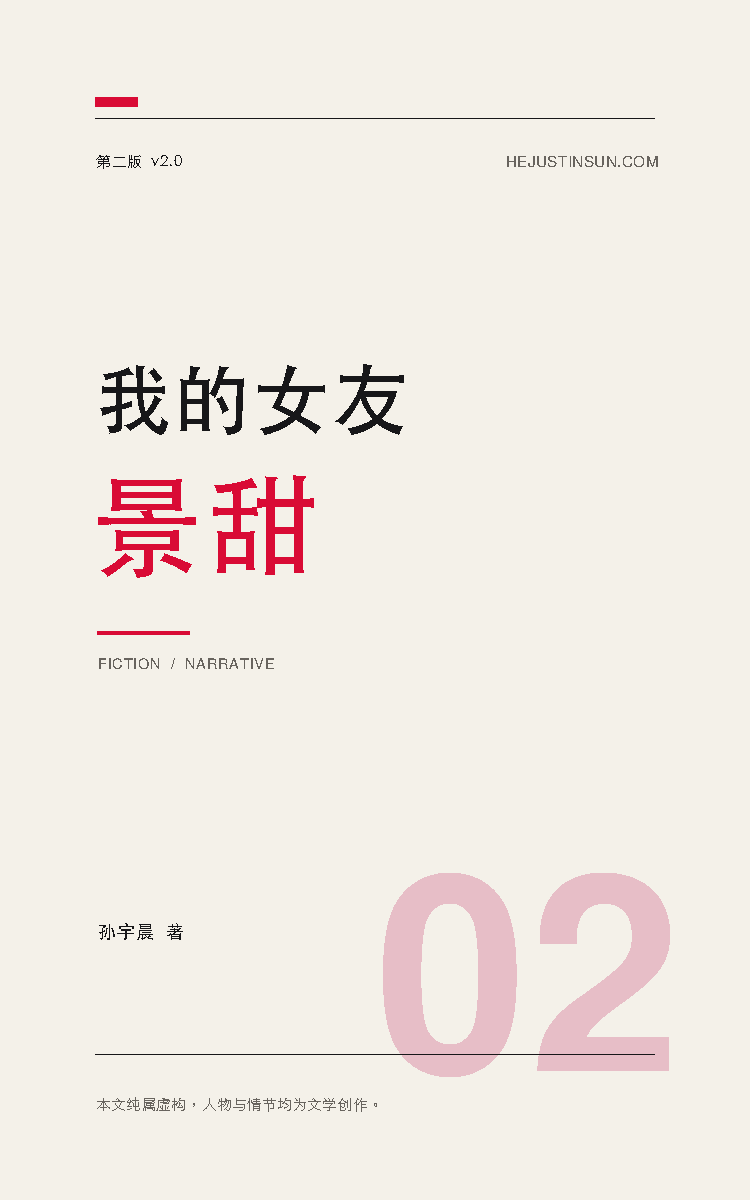
\includepdf[
  pages=1,
  fitpaper=true,
  noautoscale=true,
  pagecommand={\thispagestyle{empty}}
]{../assets/cover.pdf}

\pagenumbering{arabic}
\setcounter{page}{1}
\pagestyle{bodyrunning}
\thispagestyle{bodyopening}
% Opening-page breathing room.
\vspace*{70.817pt}

\StoryParagraph{3}{卵子ひとつの重さは、三・五マイクログラム。}

\StoryParagraph{3}{現金五千万ドルの重さは、二・五トン。}

\StoryParagraph{3}{景甜（チン・ティエン）がモンタージュ・ラグナビーチからの電話で僕に求めたのは後者で、担保に差し出したのは前者だった。}

\StoryParagraph{3}{彼女がそこへ行ったのは採卵のためだった。代理出産の子どもは2027年に生まれる予定で、早ければぎりぎり午年に間に合う。それは彼女から言い出したことだった。クリニックに着くと、彼女は言った。五千万がなければ、採らない。}

\UnprintedPause

\StoryParagraph{0}{モンタージュ・ラグナビーチは海崖の上にあり、下は太平洋だ。あのフロアを丸ごと借り切って、三十日、百万ドル。彼女のプライバシーのためだった。彼女は八日で出ていった。}

\StoryParagraph{0}{残りの二十二日間、ホテルの清掃係は毎日変わらず上がっていった。僕のアシスタントが話してくれた。鍵を返しに行ったとき、一度見かけたのだという。メキシコ人の女が台車を押し、一室ずつ入って、タオルを替え、台を拭き、布団の角を整え、出てきてドアを閉める。フロア全部を終えるのに、二時間。}

\StoryParagraph{0}{アシスタントは女に訊いた。誰も泊まっていないのに、なぜまだやるのか。}

\StoryParagraph{0}{女は言った。帳簿には、いることになっているから。}

\StoryParagraph{0}{女王を失ったヴェルサイユ宮殿。}

\StoryParagraph{0}{僕は不意に気づいた。景甜はこれが好きなのだ。景甜は、ある場所が自分のために空いていることが好きなのだ。何も起こらない。}

\StoryParagraph{3}{モンタージュ・ラグナビーチとともに空いたままだったものが、もうひとつある。ガルフストリームG700が一機、Van Nuysに気まずく駐機したまま、乗務員は毎日変わらず出勤していた。}

\StoryParagraph{3}{八日目に彼女はあの電話をかけた。それきり、誰も彼女を見ていない。}

\NarrativeBreak

\StoryParagraph{0}{2007年、すでに彼女のために金を燃やす者がいた。その年、僕は北京大学に入ったばかりだった。}

\StoryParagraph{3}{もちろん、金を燃やしていたのは僕ではない。}

\StoryParagraph{3}{QQにウィンドウがポップアップした。広告のモデルは彼女だった。あのレノボIBMの古いマシンの上で、解像度はひどくぼやけていた。僕はその画像を保存した。}

\StoryParagraph{3}{僕は家賃が年に千元の北京大学の寮でネットにつなぎ、校内網（中国版Facebook）で彼女を見つけて、友達申請を送った。校内網はひとことメッセージを書く欄があって、僕は書いては消し、消しては書き、四十分ほどかけて、最後に「你好」のひとことを送信した。}

\StoryParagraph{3}{彼女は承認しなかった。}

\StoryParagraph{3}{そもそも校内網を使ったことがなかったのかもしれない。}

\StoryParagraph{3}{それからの歳月、僕は何かをするたびにひとつの問いを考えていた。どこまで行けば、彼女は承認するのか。最初の十億のときに考えた。百億のときにも考えた。}

\StoryParagraph{3}{そのうち考えなくなった。人人網はとっくに潰れていた。}

\StoryParagraph{3}{僕は二度目の申請をしなかった。}

\StoryParagraph{3}{2011年、北京は寒かった。僕はダウンジャケットを買った。百五十元。この値段を覚えているのは、三日迷ったからだ。}

\StoryParagraph{3}{同じ年、彼女は製作費一億五千万の映画『戦国』に出た。スン・ホンレイ、フランシス・ン、キム・ヒソン、中井貴一、チアン・ウーは、十九年後のモンタージュ・ラグナビーチとガルフストリームG700と同じように、引き立て役として招かれた。彼らは自分がなぜここにいるのか分からず、来たからには何かが起こるはずだったが、何も起こらなかった。}

\StoryParagraph{3}{その後は一億五千万ドルの『グレートウォール』。チャン・イーモウ、アンディ・ラウ、マット・デイモン。その後はジャッキー・チェン。景甜ユニバースの名簿はどんどん長くなっていった。}

\StoryParagraph{3}{僕はそのころもうアメリカにいて、学び、起業し、ますます忙しくなっていった。変わらなかったのはひとつだけ。デバイスを替えるたび、どんなに面倒でも、あのQQの画像を移し続けたことだ。}

\StoryParagraph{3}{十九年後、名簿に僕が加わった。}

\NarrativeBreak

\StoryParagraph{3}{ローズウッドホテルで、僕らは初めて会った。彼女に会う日、僕はきっと緊張すると思っていた。}

\StoryParagraph{3}{しなかった。}

\StoryParagraph{3}{彼女は写真より痩せていて、ラフな格好で、ソファにもたれていた。彼女を見ながら、僕は不意に、自分が待っていたものが何だったのか思い出せなくなった。}

\StoryParagraph{3}{僕は彼女をカテランのバナナに連れていった。彼女は長いあいだ眺めてから、訊いた。これ、いくら。}

\StoryParagraph{3}{六百二十万ドル。}

\StoryParagraph{3}{彼女は言った。じゃあ、腐ったらどうするの。}

\StoryParagraph{3}{僕は黙った。彼女は言った。もういい、映画を観に行こう。}

\StoryParagraph{3}{僕はいいよと言った。}

\StoryParagraph{3}{彼女は言った。劇場には私たちふたりのほかに、誰もいてはだめ。}

\StoryParagraph{3}{僕はいいよと言った。}

\StoryParagraph{3}{僕は外に出て電話を一本かけた。戻ってきたとき、彼女はまだあのバナナの前に立っていた。}

\StoryParagraph{3}{映画は『ズートピア2』だった。}

\StoryParagraph{3}{ふたりだけの上映室。こういう場面はふつう、当局の検閲試写に使われる。}

\StoryParagraph{3}{僕はアシスタントに、映画館の座席を全部買い取らせた。}

\StoryParagraph{3}{チケットを買い占めて興行収入を水増しする行為を批判する記事を読んだことがある。券は売り切れなのに、観ているのはふたりだけだと。いまなら分かる。あれはたぶん、興行収入のためだけではなかったのだ。}

\StoryParagraph{3}{座席を全部買うのは難しくない。厄介なのは、すでに売れてしまったチケットだ。アシスタントとボディガードが先回りして映画館の入口に立ち、チケットを買った客が来ると、現金を差し出した。}

\StoryParagraph{3}{子ども連れの夫婦が来た。子どもはもう入口でポップコーンを高く掲げていた。}

\StoryParagraph{3}{アシスタントが札束を差し出す。子どもはなぜ入れないのか分からない。大人は金を受け取り、礼を言い、何も訊かずに、去った。}

\StoryParagraph{3}{その日、金を受け取ったのは二十六人だった。}

\StoryParagraph{3}{観終わると、彼女はWeChatのアイコンをジュディ警官に替えた。}

\StoryParagraph{3}{夜、彼女の乳房を手で揉んで、押しのけられた。}

\StoryParagraph{3}{嫌なのだと思った。手を引っ込めて、何か言おうとした。}

\StoryParagraph{3}{彼女は何も言わなかった。起き上がり、バッグから小さなポーチを探り出して、開いた。中にはひと並びの何かが入っていた。とても小さな工具のセットのようだった。}

\StoryParagraph{3}{彼女は言った。あなたの爪が刺さって痛いの。}

\StoryParagraph{3}{僕は一目見た。僕はずっと爪切りで適当に二回ほど切るだけで、縁は尖っていたが、ふだんは気にならなかった。}

\StoryParagraph{3}{彼女は言った。おいで。}

\StoryParagraph{3}{彼女は僕の手を自分の腿の上に置き、一本ずつ磨いた。}

\StoryParagraph{3}{まず粗い面。磨き終わると面を替え、また替える。しばらく磨いては持ち上げて灯りに透かし、また磨く。}

\StoryParagraph{3}{これはどれくらい磨くのかと僕は言った。}

\StoryParagraph{3}{彼女は言った。引っかからなくなるまで。}

\StoryParagraph{3}{十本の指に、彼女は一時間近くかけた。}

\StoryParagraph{3}{途中で彼女は教えてくれた。この面は形を整える、この面は艶を出す、最後の面は往復でこすってはだめ、一方向に沿って。}

\StoryParagraph{3}{僕はいいよと言った。}

\StoryParagraph{3}{磨き終わると、彼女は僕の手を裏返して眺め、ひと撫でした。}

\StoryParagraph{3}{彼女は言った。よし。}

\StoryParagraph{3}{触りなさい。どこでも好きなところを。}

\StoryParagraph{3}{途中で彼女はひとこと言った。いつか私がいなくなったら、あなたの爪を磨いてくれる人はもういないのよ。}

\StoryParagraph{3}{僕は少し笑って、何も言わなかった。}

\StoryParagraph{0}{彼女と知り合って三か月のとき、僕はある書類を作らせた。彼女のこれまでのプロジェクト、提携先、会社の持ち株、景国慶、田心愛、関連する口座のすべて、北京で借りている家、上海で買った家、そのほかいくつか。一週間で仕上がり、全部で四十数ページ。男や女とのあれこれもあったが、それが一番どうでもいいことだと僕は思った。}

\StoryParagraph{0}{中には、のちに彼女が自分から話してくれたことがいくつかあった。話の中身は、そこに書いてあることと少し違っていた。僕は言わなかった。}

\StoryParagraph{0}{ずっと話さないままのこともあった。僕も訊かなかった。}

\StoryParagraph{0}{僕は彼女の言うことを全部信じている。}

\StoryParagraph{0}{あの書類は取ってある。いまもずっと。}

\StoryParagraph{3}{だが、一文字も信じていない。}

\NarrativeBreak

\StoryParagraph{3}{彼女は言った。香港は人が多すぎて、顔がばれる。どこかへ出かけましょう。}

\StoryParagraph{3}{僕はいいよと言った。}

\StoryParagraph{3}{彼女は地図の上でテネリフェを指さした。}

\StoryParagraph{3}{僕はいいよと言った。}

\StoryParagraph{3}{僕は外に出て電話を一本かけた。戻ってきて初めて、その場所がアフリカ北西岸の沖、大西洋の上にあることを知った。翌日の昼、僕ら一行三十人は出発した。A330が空港で待っていた。}

\StoryParagraph{3}{飛行機の寝室で彼女は僕に訊いた。私の名前、いい名前だと思う。}

\StoryParagraph{3}{いい名前だと僕は言った。}

\StoryParagraph{3}{彼女は言った。パパの姓とママの姓をつなげたの。すごい偶然でしょ。}

\StoryParagraph{3}{初日から覚えていたよと僕は言った。}

\StoryParagraph{3}{彼女は僕を抱きしめて言った。これからは景甜って呼ばないで。ママって呼んで。}

\StoryParagraph{3}{いいよ、ママ。}

\StoryParagraph{3}{着陸すると機長が来て言った。ボス、島は最初、降ろしてくれませんでした。こんなに大きいプライベートジェットを見たことがないそうです。}

\StoryParagraph{3}{島でもルールは同じだ。まわりに人がいてはいけない。アシスタントが処理しに行った。誰もなぜかと訊かなかった。今回は何人だったか、僕は訊かなかった。}

\StoryParagraph{3}{リッツ・カールトンは大西洋に正対していて、ガラス窓が大きすぎた。彼女は一筋の光があっても眠れない。アシスタントが黒いガムテープで部屋じゅうを貼り固めた。外は真昼のように明るく、中は独房のように暗い。テープは日に炙られるとすぐ剥がれ、毎日貼り直した。}

\StoryParagraph{3}{アシスタントは全部で十一人。朝六時半に来て、僕らが眠ってから帰る。テープを貼るのはふたりの女の子で、ひとりが窓枠、ひとりがエアコンとコンセントの表示灯を受け持ち、貼り終えるとさらに三度確認する。テープは三十巻買い、あとから二十巻を買い足した。彼女たちは、午後三時以降に貼ったテープが一番剥がれやすいことに気づいた。そのころガラスが一番熱いからだ。それで朝に貼るように変えた。誰かに教わったのではない。自分たちで試して見つけたのだ。彼女たちは互いに議論していた。ひとつの工芸について語るように。}

\StoryParagraph{3}{彼女はそのふたりの女の子の名前を知っていた。僕は知らない。}

\StoryParagraph{3}{僕らはテイデ公園の道路脇に車を停めて夕日を見た。アシスタントが車からバラの花を運び下ろし、シャンパンを開けた。}

\StoryParagraph{3}{ママは雲海を眺めて言った。きれい。でも青海のデリンハの夕日には及ばない。}

\StoryParagraph{3}{僕は青海の人間だ。}

\StoryParagraph{3}{言わなかった。}

\StoryParagraph{3}{夜、僕らは山頂で星を見た。綿入れを着ていても寒かった。}

\StoryParagraph{3}{ママは言った。願い事をしよう。}

\StoryParagraph{3}{何を願ったのと僕は訊いた。}

\StoryParagraph{3}{ママは言った。教えない。}

\StoryParagraph{3}{ママは言った。きれいすぎる。ただ寒すぎるだけ。モルディブに行かない。}

\StoryParagraph{3}{僕は、わかったと言った。}

\StoryParagraph{3}{テネリフェは零下十五度、モルディブは二十七度。直線距離九千五百キロ、飛行十一時間。ただしモルディブの空港は小さすぎて、ワイドボディ機は途中で小型機に乗り換えなければならない。}

\StoryParagraph{3}{ママは言った。小さい飛行機はうるさい。やっぱり大きい飛行機がいい。}

\StoryParagraph{3}{モルディブへ向かう機内の寝室で、ママは僕に言った。願い事はね、あなたとの子どもがほしい、というもの。必ず代理出産で。}

\StoryParagraph{3}{なぜかは訊かなかった。痛いのが怖いのだと思っていた。}

\StoryParagraph{3}{途中でママが急に起き上がって携帯を探し、スターリンクにつないで、まずい、と言った。}

\StoryParagraph{3}{どうしたのと僕は訊いた。}

\StoryParagraph{3}{彼女は言った。私を脅そうとしてる人がいるの。三日前から訊いてくるのに、ずっと返してない。}

\StoryParagraph{3}{いくら要るのと僕は言った。}

\StoryParagraph{3}{あなたは構わないでと彼女は言った。}

\StoryParagraph{3}{彼女は長いあいだ文字を打っていた。消しては直し、直しては消し。打ち終わると携帯を腿の上に伏せ、しばらくするとまた裏返して見た。}

\StoryParagraph{3}{相手は誰なのと僕は訊いた。}

\StoryParagraph{0}{彼女は言った。昔いっしょにやってた人。経理で、中に入った。罪をかぶってくれたの。}

\StoryParagraph{3}{出てきて行き場がなくて、どうしても私を頼るしかない。}

\StoryParagraph{3}{いっそ警察に突き出せばいいと僕は言った。}

\StoryParagraph{3}{彼女は僕を一瞥した。あなたには分からない。}

\StoryParagraph{3}{払ったのかと僕は訊いた。}

\StoryParagraph{3}{払ったと彼女は言った。}

\StoryParagraph{3}{いくら。}

\StoryParagraph{3}{八万。}

\StoryParagraph{3}{それで三日も考えるのかと僕は言った。}

\StoryParagraph{3}{彼女は何も言わなかった。}

\StoryParagraph{3}{その日の残りの時間、彼女はほとんど口をきかなかった。着陸してからやっと眠った。}

\StoryParagraph{0}{ソネバジャニに最初に着いたのは、ママのトランクだった。三十人分の荷物は小型機に載りきらず、三機に分けた。ママのトランクはひとつだけなのに、単独で一機。ほかの人のと一緒にしないで、と彼女は言った。}

\StoryParagraph{0}{ソネバジャニは no news, no shoes で名高く、ママは安心した。}

\StoryParagraph{3}{ホテルのバトラー、ボディガード、アシスタント、あわせて二十六人。さらにドローン操縦士がふたり、遠くからついてくる。アシスタントたちはまたテープを貼りはじめた。エアコンの灯、コンセントの灯、何度も何度も。}

\StoryParagraph{0}{夜、僕らは暗号を交換するように互いの昔の恋人を交換した。王朝が元号を照合するように。ママはいかなる手違いも許さなかった。ただ、ママにはひとつ禁句があった。あのアスリートのことは口にできない。}

\StoryParagraph{0}{僕は口にしなかった。ママの背中のタトゥーが、アスリートのために彫られたものだと知ってはいたけれど。}

\StoryParagraph{3}{たぶん大きすぎて、消せないのだ。}

\StoryParagraph{0}{彼女は言った。もう私たち家族なんだから。パパとママが私をここまで育てるのは大変だったの。結納金を出してね。}

\StoryParagraph{0}{僕はいいよと言った。}

\StoryParagraph{0}{彼女はふたつの名前を挙げた。景国慶、田心愛。そしてふたつの口座番号。}

\StoryParagraph{0}{三千万、人民元。}

\StoryParagraph{0}{僕は振り込んだ。そのふたつの名前を、僕はあの四十数ページで初めて見たのだった。}

\StoryParagraph{3}{しばらくして、彼女は携帯を差し出して僕に見せた。田心愛は二文字だけ返してきた。「了解」。}

\StoryParagraph{0}{あるときママは言った。私がこういうものを欲しがるとき、何を考えてるか知ってる。}

\StoryParagraph{0}{何、と僕は言った。}

\StoryParagraph{0}{彼女は言った。あなたが一度でも、いやだと言うことはないのかなって。}

\StoryParagraph{0}{ないよと僕は言った。}

\StoryParagraph{0}{彼女は言った。それじゃ、つまらない。}

\StoryParagraph{3}{僕は思った。僕にできないことなど、あるだろうか？}

\StoryParagraph{0}{退屈しきったとき、僕はあの2007年のQQの画像をいじって、新しいデバイスに移そうとしていた。ママが頭を寄せてきた。私に隠れてよその女の写真を保存してるの、これは誰。}

\StoryParagraph{0}{僕は黙った。何も言わなかった。}

\StoryParagraph{0}{彼女は画像がぼやけすぎだと言って、別のことをしに行った。}

\StoryParagraph{0}{その晩、僕はその画像を消した。}

\StoryParagraph{3}{翌日、古い携帯から復元した。}

\StoryParagraph{0}{ママも携帯を延々とスクロールしていた。何を見てるのと僕は訊いた。}

\StoryParagraph{0}{彼女は言った。なんでもない。トップクレジット争いの、くだらない話。}

\StoryParagraph{0}{トップクレジット争い。一本の映画で一番手に名前を出せるスターはひとりしかいない。主演の男と女でも、先頭に立てるのはひとりだけだ。}

\StoryParagraph{0}{くだらないなと僕は言った。}

\StoryParagraph{0}{彼女は言った。そうね。もっとつらいのはね、ときどき撮影所夫婦っていうのがあって、組に入ったら四、五十日、ずっと同じ男と芝居をして、夜はセックスして、昼はトップクレジットを争うの。}

\StoryParagraph{0}{人間の本性に反しすぎると僕は言った。}

\StoryParagraph{0}{そうねと彼女は言った。}

\StoryParagraph{0}{でも撮影が終われば、それまで何回セックスしていようと、すべて何もなかったことにするの。}

\StoryParagraph{3}{それから彼女はまた三十分、画面を見ていた。}

\StoryParagraph{0}{2026年1月2日、ソネバジャニ。新しい年、僕はママに求婚した。}

\StoryParagraph{0}{決めたのは1月1日の朝だった。指輪は香港にある。島には指輪を売る店がない。アシスタントが水上飛行機でマレへ行き、午後に戻ってきた。指輪はホテルの封筒に入っていた。}

\StoryParagraph{0}{ママは言った。ダイヤが小さすぎる。}

\StoryParagraph{0}{ママは言った。いいの、あとで大きいのを埋め合わせて。}

\StoryParagraph{0}{それと、北京に来られる？}

\StoryParagraph{0}{僕は黙った。}

\StoryParagraph{0}{彼女は、僕が行きたくないのだと思った。}

\StoryParagraph{0}{ママは言った。どうして私にこんなに良くしてくれるの。}

\StoryParagraph{0}{君が好きだからだと僕は言った。}

\StoryParagraph{0}{彼女は言った。じゃあ、前はほかの人にもこうだったの。}

\StoryParagraph{0}{なかったと僕は言った。}

\StoryParagraph{3}{彼女は少し笑って、何も言わなかった。}

\StoryParagraph{0}{ある朝、僕は早く目が覚めた。彼女はベッドにいなかった。}

\StoryParagraph{0}{出てみると、彼女は露台に座って海に向かっていた。海全体が黒かった。灯りはつけず、まだ夜は明けていない。}

\StoryParagraph{0}{こんなに早く起きてどうしたのと僕は訊いた。}

\StoryParagraph{0}{彼女は言った。日数を数えてるの。}

\StoryParagraph{0}{何を数えるのと僕は言った。}

\StoryParagraph{0}{彼女は言った。戻って寝てて。}

\StoryParagraph{0}{僕はしばらく彼女の隣に座っていたが、何を言えばいいのか分からなかった。それから戻って眠った。}

\StoryParagraph{3}{次に目が覚めたとき、彼女はもう化粧を終えていた。}

\StoryParagraph{0}{モルディブに十四日いて、彼女に気づいた者はひとりもいなかった。}

\StoryParagraph{0}{十三日目の夜、レストランで、彼女はサングラスを外した。しばらくして、帽子も脱いで、テーブルに置いた。彼女はそのまま食事のあいだじゅう座っていた。隣のテーブルはドイツ人の老夫婦で、ウェイターはスリランカ人。誰ひとり、彼女を余計に見なかった。}

\StoryParagraph{0}{食べ終わると、彼女は帽子をかぶり直した。}

\StoryParagraph{0}{ママは言った。帰ろう。}

\StoryParagraph{0}{まだ足りないんじゃなかったのかと僕は言った。}

\StoryParagraph{3}{彼女は言った。静かすぎる。}

\UnprintedPause

\StoryParagraph{0}{香港に戻って、ママは僕の両親に会った。}

\StoryParagraph{0}{その夜、彼女は言った。家では両家の顔合わせと結婚の支度をするから、できるだけ多く包んで。振込先はやはり景国慶と田心愛。}

\StoryParagraph{0}{なぜかは訊かなかった。}

\StoryParagraph{0}{カード一枚の一日の限度額は百万だと僕は言った。}

\StoryParagraph{0}{ママは遅すぎると言った。}

\StoryParagraph{0}{五枚で振り込んで。}

\StoryParagraph{0}{五枚のカード、ふたつの口座、順繰りに振り込む。三枚目に差しかかったとき、僕は一瞬ためらった。それでも最後まで振り込んだ。}

\StoryParagraph{3}{ママは言った。効率が悪すぎる。}

\StoryParagraph{0}{正月は、うちの親たちを香港に呼んで一緒に過ごそうよと僕は言った。}

\StoryParagraph{0}{ママは言った。今年はもう海南で年越しって決まってるの。来年ね。}

\StoryParagraph{0}{春節、ビクトリア・ハーバーに花火が上がり、百万人が来た。彼女はいなかった。}

\StoryParagraph{0}{明け方三時、僕は両親を送り届けた。}

\StoryParagraph{0}{道はがらんとして、赤信号には一台の車も待っていなかった。それでも僕は停まった。}

\StoryParagraph{0}{ママは言った。しばらく会えない。すぐロサンゼルスへ採卵に行くの。手元のことを先に片づけないと。}

\StoryParagraph{0}{ママはまた訊いた。北京に来られる？}

\StoryParagraph{0}{僕は黙った。}

\StoryParagraph{3}{北京に何があるのか、彼女は言わなかった。僕も訊かなかった。}

\StoryParagraph{0}{ママは言った。香港に家を一軒買って。名義は私で。}

\StoryParagraph{0}{僕は、わかったと言った。}

\StoryParagraph{3}{バレンタインデーも会わなかった。}

\StoryParagraph{0}{あるとき彼女は電話で言った。今朝、採血を八本もされた。}

\StoryParagraph{0}{そんなにと僕は言った。}

\StoryParagraph{0}{平気と彼女は言った。}

\StoryParagraph{0}{お疲れさまと僕は言った。}

\StoryParagraph{0}{それから僕らは別の話をした。}

\StoryParagraph{0}{あとになって知った。あの採血は空腹で受けなければならず、月経周期の二日目か三日目、日にちを間違えてはいけない。あの朝、彼女はたぶん六時には家を出た。北京の冬、まだ夜は明けていない。検査はその後どんどん増えた。僕がこのことを知ったのは、アシスタントの毎月の支払一覧に一項目が増えたからだ。最初に現れたのは去年で、金額は大きくない、数千元。それから毎月あって、ときには二、三件。僕の決裁は速かった。この程度の金額に明細は要らないのだ。あとで知った。あれは採血、ホルモン六項目、超音波、AMH。彼女にどれだけ残りがあるのか、いくつ採れるのか、先へ進む値打ちがあるのかを見るためのものだった。}

\StoryParagraph{0}{それはぜんぶ北京でやったことだ。}

\StoryParagraph{3}{どこの病院かは知らない。ひとりで行ったのか、誰かが付き添ったのかも知らない。}

\StoryParagraph{0}{2月25日、彼女は香港に降り立った。}

\StoryParagraph{0}{彼女は言った。ロサンゼルスへは行かない。先に香港の家を見ないかぎり。}

\StoryParagraph{0}{僕は半年のあいだに見た十数軒の家をぜんぶ送った。彼女はどれも気に入らなかった。その十数軒に、僕は一軒も行ったことがない。アシスタントが半年かけて一軒ずつ選び、アシスタントが僕に転送し、僕が彼女に転送した。一軒はミッドレベルズにあって、動画にはビクトリア・ハーバーが映っていた。撮ったのは夕暮れ。一瞬レンズが揺れて、撮っている人の影が壁に映り込んだ。その影を見ながら僕は思った。この人は誰だろう。今日どれだけ歩き、何軒の家を見たのだろう。この家を誰に見せるためのものか、知っているのだろうか。}

\StoryParagraph{3}{時間が足りず、彼女は結局ロサンゼルス行きのG700に乗った。2月28日、モンタージュ・ラグナビーチに着いた。}

\NarrativeBreak

\StoryParagraph{0}{八日目にママは電話をかけてきた。向こうは午後、こちらは明け方だった。}

\StoryParagraph{0}{彼女は言った。五千万、ドルで。}

\StoryParagraph{0}{僕は言った。少し考えさせて。}

\StoryParagraph{0}{彼女は何も言わなかった。向こうに海の音が聞こえた。}

\StoryParagraph{0}{しばらくして彼女は言った。いいわ。}

\StoryParagraph{0}{彼女は電話を切った。}

\StoryParagraph{3}{彼女と知り合ってから、彼女に「少し考えさせて」と言ったことは一度もなかった。}

\StoryParagraph{0}{僕はClaude CodeにAPIを読ませて、現金資産をすべて洗い出した。結論は、僕には何の影響もないということだった。もう一度確かめた。僕はClaude Codeに問いを打ち込んだ。Claudeは言った。この五千万ドルを彼女に渡してはいけない。}

\StoryParagraph{3}{僕は訊いた。彼女はもう僕を愛していないのか？}

\StoryParagraph{3}{Claudeは言った。愛については、関心もないし、理解もしない。だが、この五千万ドルを彼女に渡してはいけない。}

\StoryParagraph{3}{僕は一度も彼女を拒んだことがない。気前の良さではない。恐怖だ。次の一秒の答えが怖いのだ。}

\StoryParagraph{0}{それをいま、誰かが代わりに言ってくれた。}

\StoryParagraph{0}{僕はその一行を長いあいだ見つめていた。ぞっとしたのは、それが賢いからではない。Claudeに一片のためらいもなかったからだ。}

\StoryParagraph{0}{それは苦しまない。}

\StoryParagraph{0}{そのとき僕は思った。これはたぶん、もっと高いところにある何かだ。人間にはこうはできない。}

\StoryParagraph{3}{彼女はもう僕を愛していないのか。}

\StoryParagraph{3}{翌日、彼女はかけ直してきた。}

\StoryParagraph{3}{ママは言った。海が大きい。}

\StoryParagraph{3}{そうなの、と僕は言った。}

\StoryParagraph{3}{彼女は言った。このフロアは広すぎて、声が響くの。朝、掃除の人が来ると、私はバスルームに隠れて、いなくなるのを待つの。}

\StoryParagraph{3}{来させないようにもできるよと僕は言った。}

\StoryParagraph{3}{彼女は、いらない、と言った。}

\StoryParagraph{3}{彼女は言った。クリニックがね、お子さんのお父さんはいつ来るのかって。}

\StoryParagraph{3}{人をやろうかと僕は言った。}

\StoryParagraph{3}{彼女は言った。いらない。}

\StoryParagraph{3}{それから彼女は言った。決めたの。}

\StoryParagraph{3}{僕は何も言わなかった。考えていたのではない。何も考えていなかった。電話の向こうには海があり、こちらにはビクトリア・ハーバーがあり、どちらも黙っていた。数えてみた。十一秒。}

\StoryParagraph{3}{景甜は言った。いい。}

\StoryParagraph{3}{景甜は言った。わかった。}

\StoryParagraph{3}{彼女は電話を切った。}

\StoryParagraph{3}{あの二日間、五千万のほかに彼女が何を言ったか、あとから数えきれないほど思い返した。海が大きい。このフロアは広すぎる。バスルームに隠れている。それだけだ。全部覚えている。一字も違えず。思い出せないのは彼女の声だ——「わかった」と言ったとき、どんな口調だったのか。}

\StoryParagraph{0}{思い出せない。そのうち、思い返すのをやめた。}

\StoryParagraph{0}{僕は携帯をナイトテーブルに置いた。画面を下に向けて。それからひとつのことをした。なぜだかいまも分からない。手を胸に当てて、数えたのだ。}

\StoryParagraph{0}{心拍は安定していた。}

\StoryParagraph{0}{もう一度数えた。やはり安定していた。一分間に六十いくつ。ふだんと変わらない。僕はそこに座り、自分の胸を手で押さえていた。医者が他人を診察するように。}

\StoryParagraph{3}{僕は思った。そうか、こういうことか。}

\StoryParagraph{0}{その日の残りの時間、僕は何もしなかった。部屋にこもったまま日が暮れ、また夜が明けるまで、ビクトリア・ハーバーが青から灰色に、灰色から黒に変わっていくのを眺めていた。朝六時、ハーバーの対岸の金融センターが、一棟また一棟と灯りをともし始めた。途中でアシスタントが一度ドアをノックして、夕食はどうするかと訊いた。要らないと僕は言った。}

\StoryParagraph{3}{僕は泣かなかった。ずっと、自分が泣くのを待っていた。}

\NarrativeBreak

\StoryParagraph{0}{のちにアシスタントが精算に来た。その中に、テネリフェのホテルへの賠償という一項があった。僕らが発ったあとも、テープは数日貼られ続けた。もう貼らなくていいと、誰も彼女たちに言わなかったのだ。ホテルによれば、貼った期間が長すぎ、回数が多すぎて、窓枠の糊の痕が落ちない。あのガラスは一枚まるごと交換になるという。}

\StoryParagraph{0}{承認したと僕は言った。}

\StoryParagraph{3}{あのガラスは大西洋に面している。}

\StoryParagraph{0}{請求書の燃油の項目は、モンタージュのあのフロアより高かった。訊いてみた。アシスタントは言った。A330は二百人乗りとして設計されていて、うちは三十人しかいない。軽すぎて、離陸のトリムが合わない。だから毎回余分に給油して、十分に重くなるまで積む。着いたら、余分に積んだ分は残しておけないので、抜いて捨てる。}

\StoryParagraph{0}{僕は言った。毎回そうなのか？}

\StoryParagraph{3}{毎回そうです、と彼は言った。}

\StoryParagraph{0}{それから、ロサンゼルスのクリニックから送り返されてきた箱がひとつ。八日分の排卵誘発剤の注射、要冷蔵、一本も開封されていない。}

\StoryParagraph{3}{それから代理出産エージェンシーの手付金、二十万ドル、返金不可。代理母は一月にはもう決まっていた。カリフォルニアの人、三十四歳、出産経験二回。ファイルに写真があったが、僕は見ていない。彼女は一月には準備ができていたのだ。}

\StoryParagraph{3}{景甜が去ったあと、僕はあの2007年の画像をもう一度引っぱり出して見た。十九年。デバイスの画素はどんどん上がっていくのに、この画像はまるで画素がどんどん下がっていくようで、顔はぼやけている。長いあいだ拡大して眺め、彼女とその後の彼女とでどこが違うのか探した。ひとつも見つからなかった。あの画像は、もともとよく見えないのだから。}

\StoryParagraph{0}{ある日、爪切りで爪を切って、切り終えて触ってみると、尖っていた。}

\StoryParagraph{0}{引き出しにあれがまだあることを思い出した。彼女が残していったものだ。}

\StoryParagraph{0}{取り出して二度ほど磨いた。違う。一方向に沿って、と彼女は言っていた。どちらの方向だったか、忘れてしまった。}

\StoryParagraph{0}{僕はそれを元に戻した。}

\StoryParagraph{3}{僕の爪はいまも人を引っかく。}

\StoryParagraph{0}{ある朝、携帯にリマインダーが表示された。去年、アシスタントがスケジュールを組んだときに設定したものだ。出産予定日の三か月前、部屋の準備。}

\StoryParagraph{3}{僕はそれを消した。}

\StoryParagraph{0}{彼女が去ってから、僕はずっとひとつのことを考えている。}

\StoryParagraph{0}{あの日、渡していたら、彼女は残っただろうか。}

\StoryParagraph{0}{長いあいだ考えた。}

\StoryParagraph{3}{そのうち僕はあの書類を取り出して、もう一度読んだ。四十数ページ。}

\StoryParagraph{0}{それから春節の夜のことを思い出した。最上階から、香港のビクトリア・ハーバーの花火を見下ろしていた。}

\StoryParagraph{0}{百万人が潮のように押し寄せ、花火が終わると、百万人が引いていく。}

\StoryParagraph{0}{百万人。}

\StoryParagraph{0}{毎年こうなのだ。}

\StoryParagraph{0}{明け方三時の香港では、}

\StoryParagraph{3}{何も起こらなかった。}

\end{document}
